\subsection{DDoS}
This subsection reveals more granular data about the DDoS dataset.

\subsubsection{Accuracy}
Figure~\ref{fig:ddos_accuracy} shows the accuracy of different compressors, metrics, and sample selection methods.

\begin{figure}[h!]
	\centering
    \captionsetup[subfigure]{skip=0pt}
	\begin{subfigure}[t]{.44\textwidth}
		\centering
		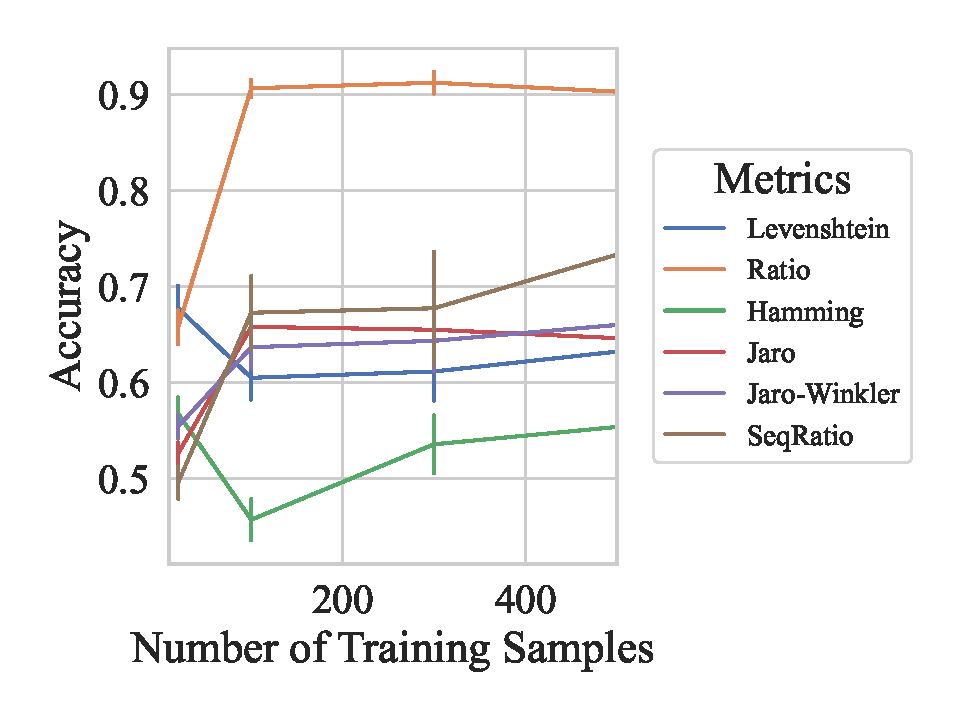
\includegraphics[width=\textwidth]{figs/ddos/string_metric_vs_accuracy.pdf}
	\end{subfigure}
	~
	\begin{subfigure}[t]{.44\textwidth}
		\centering
		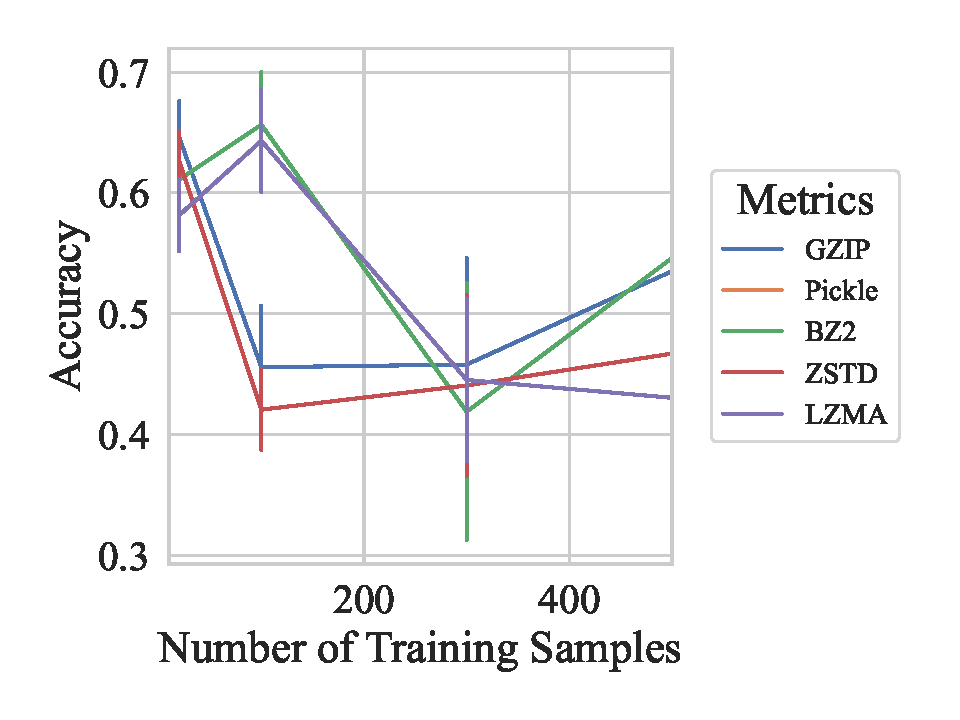
\includegraphics[width=\textwidth]{figs/ddos/compressor_metric_vs_accuracy.pdf}
	\end{subfigure}
	\caption{Accuracy across different different string kernel metrics (left), and compression methods (right).}
	\label{fig:ddos_accuracy}
\end{figure}

\subsubsection{Training Time}

Figure~\ref{fig:ddos_training_time} depicts the training time across all the tested compressors, distance metrics, and sample selection methods.

\begin{figure}[h!]
    \centering
    \captionsetup[subfigure]{skip=0pt}
	\begin{subfigure}[t]{.44\textwidth}
		\centering
		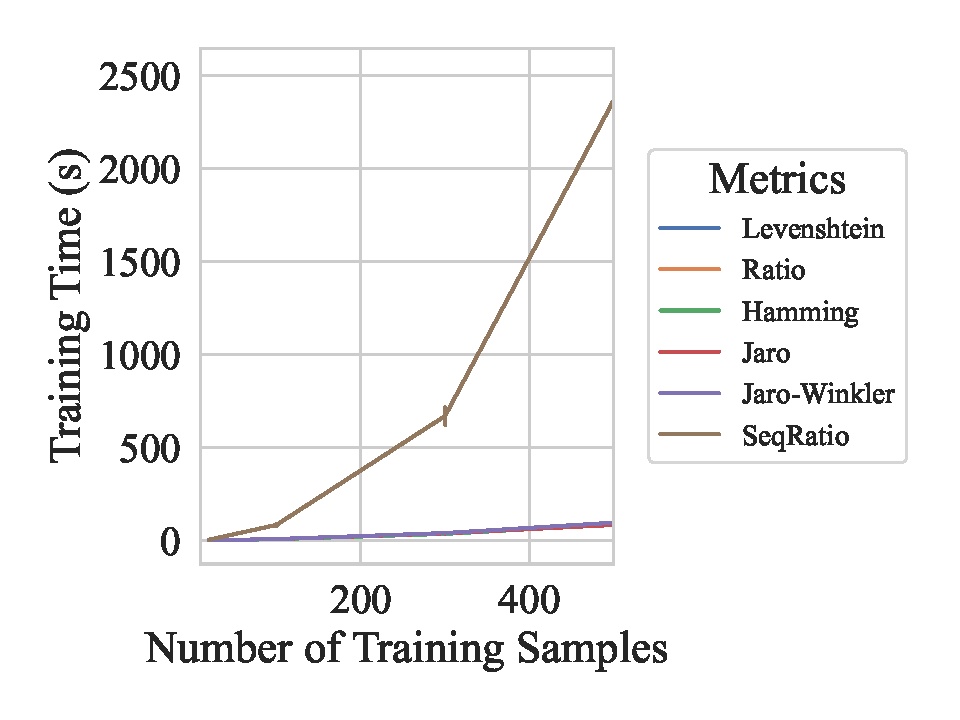
\includegraphics[width=\textwidth]{figs/ddos/string_metric_vs_train_time.pdf}
	\end{subfigure}
	~
	\begin{subfigure}[t]{.44\textwidth}
		\centering
		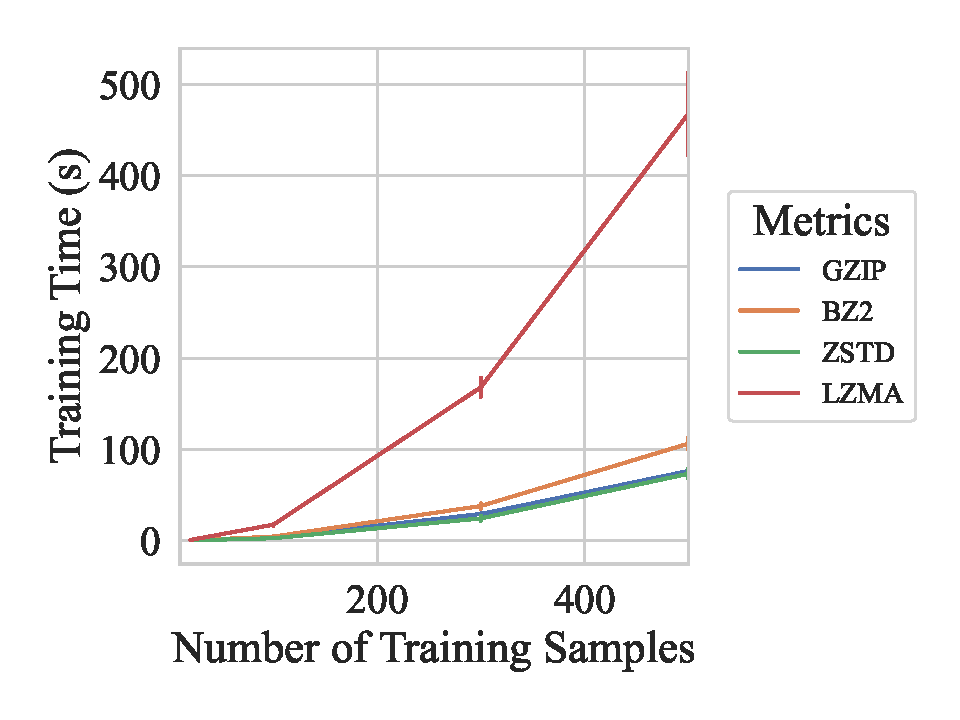
\includegraphics[width=\textwidth]{figs/ddos/compressor_metric_vs_train_time.pdf}
	\end{subfigure}
	\caption{Training time across different different string  metrics (left), and compression methods (right).}
	\label{fig:ddos_training_time}
\end{figure}

\subsubsection{Prediction Time}

Figure~\ref{fig:ddos_prediction_time} shows the prediction time of different compressors, metics, and sample selection methods.
\begin{figure}[h!]
	\centering
    \captionsetup[subfigure]{skip=0pt}
	\begin{subfigure}[t]{.44\textwidth}
		\centering
		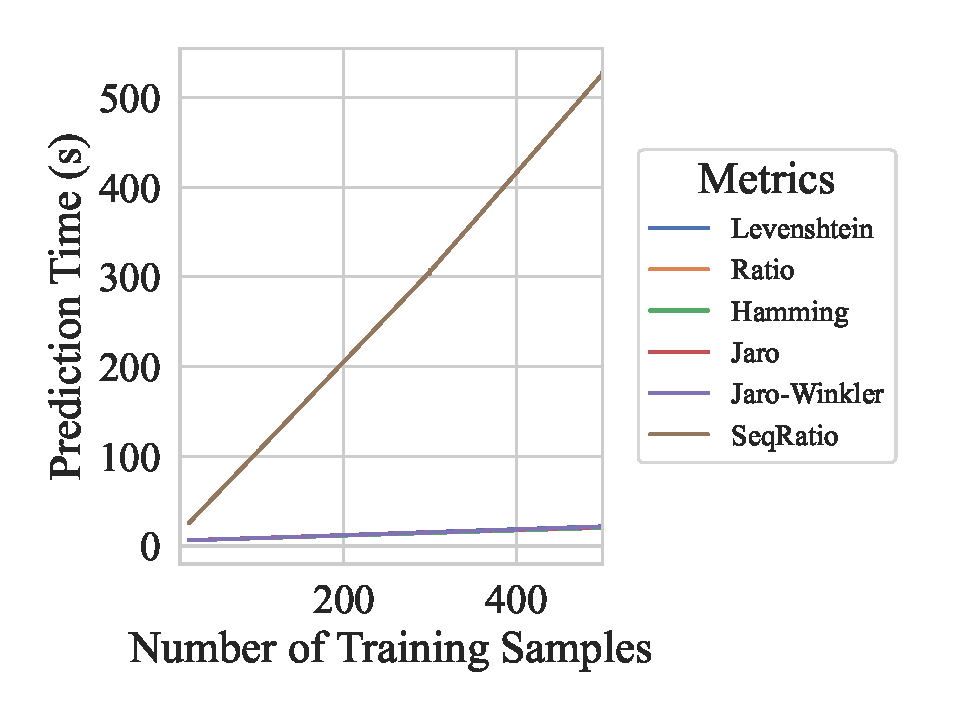
\includegraphics[width=\textwidth]{figs/ddos/string_metric_vs_predict_time.pdf}
	\end{subfigure}
	~
	\begin{subfigure}[t]{.44\textwidth}
		\centering
		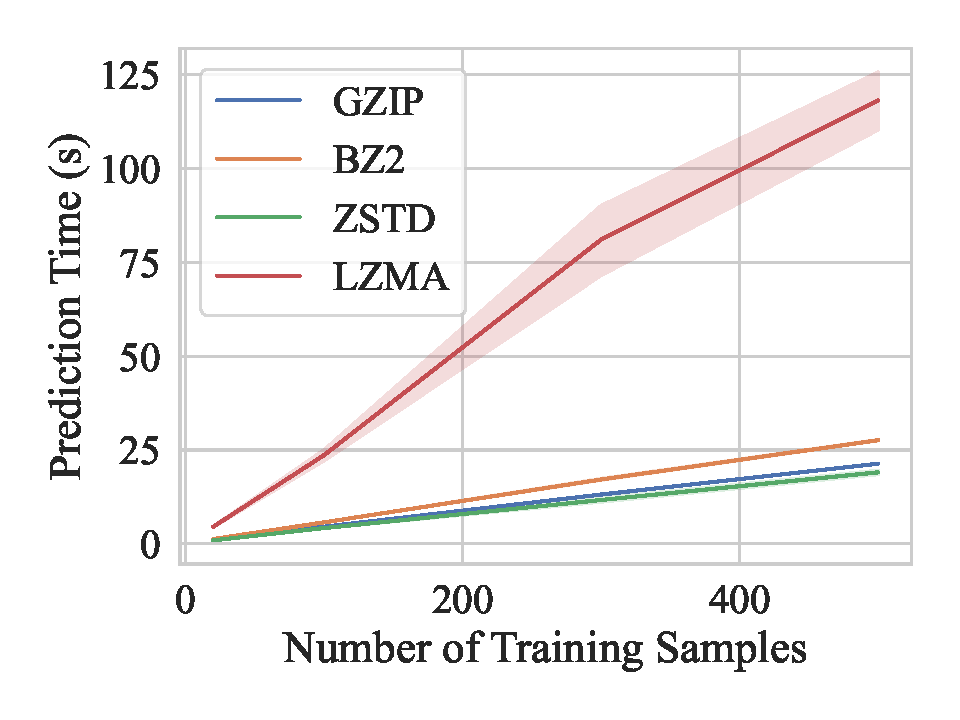
\includegraphics[width=\textwidth]{figs/ddos/compressor_metric_vs_predict_time.pdf}
	\end{subfigure}
	\caption{Prediction time across different different string metrics (left), and compression methods (right).}.
	\label{fig:ddos_prediction_time}
 
\end{figure}

\subsubsection{Symmetry}

Figure~\ref{fig:ddos_symmetry} shows the effect of assuming symmetry for different models and distance metrics.

\begin{figure}[h!]
    \centering
    \captionsetup[subfigure]{skip=0pt}
    \begin{subfigure}[t]{.44\textwidth}
        \centering
        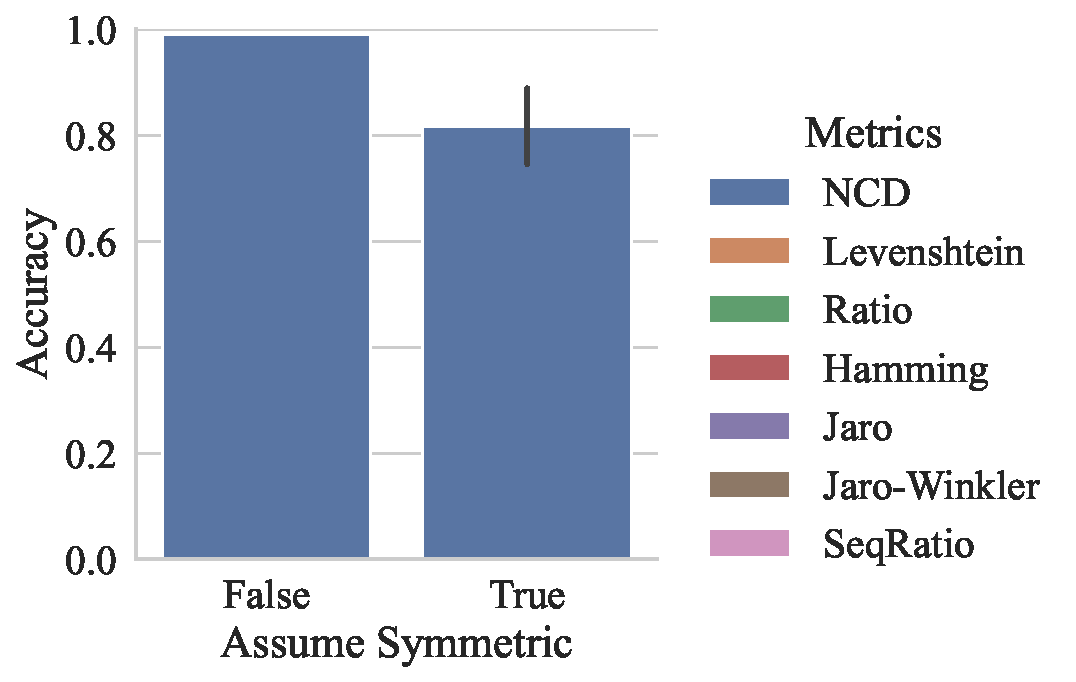
\includegraphics[width=\textwidth]{figs/ddos/symmetric_vs_metric.pdf}
    \end{subfigure}
    \begin{subfigure}[t]{.44\textwidth}
        \centering
        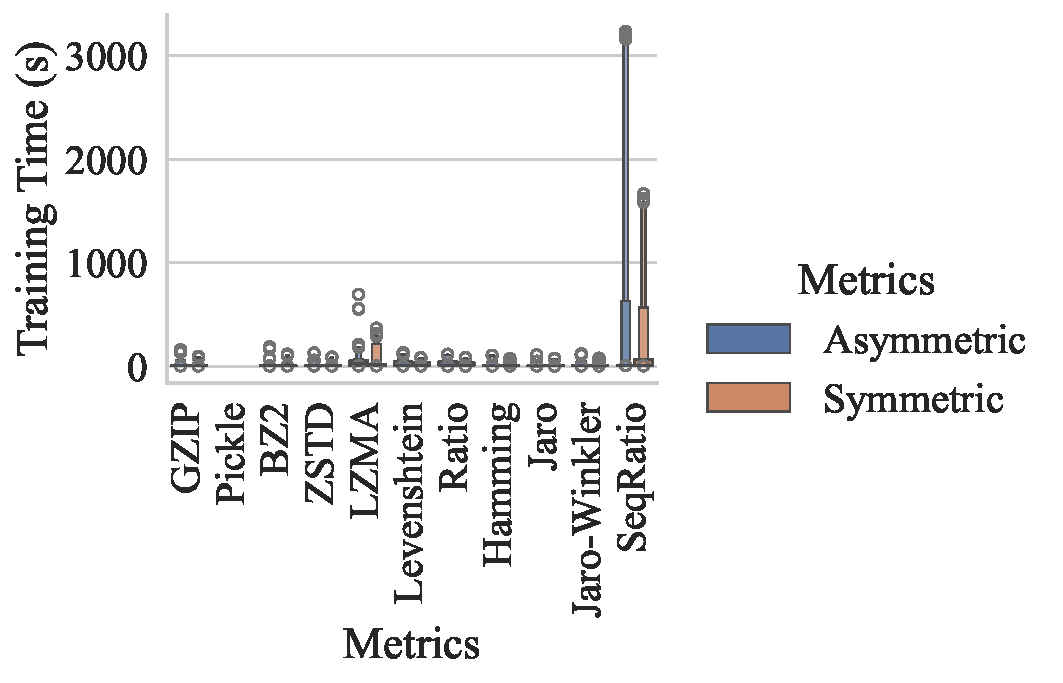
\includegraphics[width=\textwidth]{figs/ddos/symmetric_vs_metric_train_time.pdf}
    \end{subfigure}
    \caption{Accuracy across (left) and prediction time (right) across several compression methods and distance metrics with and without assuming symmetric distances.}
    \label{fig:ddos_symmetry}
\end{figure}